\documentclass[Letter,11pt]{article}
\usepackage[utf8x]{inputenc}
\usepackage{amsmath}
\usepackage{graphicx}
\usepackage[margin=1in]{geometry}
\graphicspath{{Pictures/}}
\usepackage[colorinlistoftodos]{todonotes}
\usepackage{listings}
\usepackage[american voltages, americancurrents,siunitx]{circuitikz}
\usepackage{pgfgantt}
\usepackage{lscape}
\usepackage{tikz-er2}
\usepackage{fast-diagram}
\usepackage{tikz}
\usepackage{multirow}
\usepackage{xcolor,colortbl}
\usepackage{array}
\usepackage{hhline}
\usepackage{helvet}
\renewcommand{\familydefault}{\sfdefault}
\usetikzlibrary{shapes.geometric,arrows,automata,calc,shapes, positioning}


\newcommand{\labs}{\renewcommand{\chaptername}{Lab}}
\newcommand{\Appendix}{	\makeatletter 
					\appendix
					\renewcommand\chaptername{Appendix}}

\NewDocumentCommand{\rot}{O{45} O{1em} m}{\makebox[#2][l]{\rotatebox{#1}{#3}}}%
\newcolumntype{M}{>{\centering\arraybackslash}m}

\lstset{language=C,
	numbers=left,
	keywordstyle=\color{kewordPurple},
	stringstyle=\color{stringBlue},
	commentstyle=\color{comentGreen},
	morecomment=[l][\color{magenta}]{\#}}

%
% colors
%
\definecolor{kewordPurple}{RGB}{127,0,85}
\definecolor{comentGreen}{RGB}{63,127,95}
\definecolor{stringBlue}{RGB}{42,0,255}
%http://brand.msu.edu/design-visual/index.html
\definecolor{MSUgreen}{RGB}{23,69,59}
\definecolor{othergreen}{RGB}{13,177,75}
\definecolor{MSUgray}{RGB}{153,162,162}
\definecolor{MSUorange}{RGB}{240,133,33}
\definecolor{MSUgreenBlue}{RGB}{0,129,131}
\definecolor{MSUgreenBlue}{RGB}{0,129,131}
\definecolor{MSUBlueGray}{RGB}{144,154,183}
\definecolor{MSUDarkGray}{RGB}{83,80,84}
\definecolor{MSULimeGreen}{RGB}{209,222,63}
\definecolor{MSUTan}{RGB}{232,217,181}
\definecolor{MSUTanDark}{RGB}{200,154,88}
\definecolor{MSUOffGreen}{RGB}{148,174,74}
\definecolor{MSUPurple}{RGB}{110,0,95}
\definecolor{MSUDarkorange}{RGB}{203,90,40}



\begin{document}
	%make the tile
	%%%%%%%%%%%%%%%%%%%%%%%%%%%%%%%%%%%%%%%%%
% University Assignment Title Page 
% LaTeX Template
% Version 1.0 (27/12/12)
%
% This template has been downloaded from:
% http://www.LaTeXTemplates.com
%
% Original author:
% WikiBooks (http://en.wikibooks.org/wiki/LaTeX/Title_Creation)
%
% License:
% CC BY-NC-SA 3.0 (http://creativecommons.org/licenses/by-nc-sa/3.0/)
% 
% Instructions for using this template:
% This title page is capable of being compiled as is. This is not useful for 
% including it in another document. To do this, you have two options: 
%
% 1) Copy/paste everything between \begin{document} and \end{document} 
% starting at \begin{titlepage} and paste this into another LaTeX file where you 
% want your title page.
% OR
% 2) Remove everything outside the \begin{titlepage} and \end{titlepage} and 
% move this file to the same directory as the LaTeX file you wish to add it to. 
% Then add \input{./title_page_1.tex} to your LaTeX file where you want your
% title page.
%
%%%%%%%%%%%%%%%%%%%%%%%%%%%%%%%%%%%%%%%%%
	
\begin{titlepage}
		             
		\newcommand{\HRule}{\rule{\linewidth}{0.5mm}} % Defines a new command for the horizontal lines, change thickness here
		
		\center % Center everything on the page
		
		%----------------------------------------------------------------------------------------
		%	HEADING SECTIONS
		%----------------------------------------------------------------------------------------
		
		\textsc{\LARGE Michigan State University}\\[0.5cm] % Name of your university/college
		\textsc{\Large Department Of Electrical and Computer Engineering}\\[0.5cm] % Major heading such as course name
		%\textsc{\large smaller big text}\\[0.5cm] % Minor heading such as course title
		\textsc{\Large ECE 480 Senior Design}\\[0.5cm]
		
		%----------------------------------------------------------------------------------------
		%	TITLE SECTION
		%----------------------------------------------------------------------------------------
		
		\HRule \\[0.2cm]
		{ \huge \bfseries Final Project Proposal\\ ArcelorMittal USA\\ Safety Equipment Bar Code Scanner}\\[0.2cm] % Title of your document
		\HRule \\[1.5cm]
		
		%----------------------------------------------------------------------------------------
		%	AUTHOR SECTION
		%----------------------------------------------------------------------------------------
		\noindent
		\begin{minipage}[t]{0.3\textwidth}
			\begin{flushleft} \large
				\emph{Team Members:}\\
				Kyle \textsc{Inch}\\
				Alexandria \textsc{Marone}\\
				Seth \textsc{McKisson}\\
				Trevor \textsc{Sabo}\\
				Ian \textsc{Grosh}\\ % Your name
			\end{flushleft}
		\end{minipage}% A new line will break it so dont Ian!
		\begin{minipage}{0.3\textwidth}
			\centering
			{\LARGE Design Team 3}
		\end{minipage}
		\begin{minipage}[t]{0.3\textwidth}
			\begin{flushright} \large
				\emph{Facilitator:}\\  % Supervisor's Name
				%\centering
				Dr. Bingsen \textsc{Wang}
				
			\end{flushright}
			
		\end{minipage}\\[1cm]
		
		% If you don't want a supervisor, uncomment the two lines below and remove the section above
		%\Large \emph{Author:}\\
		%John \textsc{Smith}\\[3cm] % Your name
		
		%----------------------------------------------------------------------------------------
		%	DATE SECTION
		%----------------------------------------------------------------------------------------
		
		{\large \today}\\[0.5cm] % Date, change the \today to a set date if you want to be precise
		
		%----------------------------------------------------------------------------------------
		%	LOGO SECTION
		%----------------------------------------------------------------------------------------
		
		
		
		\begin{minipage}[t]{0.4\textwidth}
			\begin{center} 
			
\includegraphics{egr_logo.png}%\\[1cm]  % Include a department/university logo - this will require the graphicx package
			\end{center}
		\end{minipage}%
		\begin{minipage}[t]{0.4\textwidth}
			\begin{center} 
		
\includegraphics{MSUSealBlack1inch.png}
			\end{center}
		\end{minipage}\\[2cm]
	\begin{abstract}
		Design team three has been asked to create a system to keep track of safety equipment on ArcelorMittal's buildings. To do this the team needs to build some systems. These systems will enable administrators to both monitor compliance standards on areas they are in charge of, and make sure that safety equipment is being properly checked and documented. Reports will be sent out periodically on the above to said administrators.  On the user end, an Android application  that uses a scanner will be created that will enable users to quickly answer questions on safety equipment standards.

	\end{abstract}
		%\\[1cm] 
		% Include a department/university logo - this will require the graphicx package
		%----------------------------------------------------------------------------------------
		


		
		
		%\vfill % Fill the rest of the page with whitespace
		
\end{titlepage}

	%make the abstract
	\begin{abstract}
		Design Team 3 as been asked to create a system to keep track of  and ensure complacence for the safety equipment on Arcelormittal's buildings. To do this the team needs to build three septate systems, a collection server scripts to manage a database, generate reports, and send reminder emails. A web based application to allow administrators to add items to a database and perspective tasks.A Android application to scan bar codes and recode response to assigned question.This project proposal is broken into two parts, first the project is defined in a way that hopefully will do the fowling:\todo{This jusmps around I to much}
		\begin{enumerate}
			\item Demonstrate the teams current understanding of the project.
			\item Define the project in such a way that it will be.
			\item Demonstrate that the team has internalized the design challenge faced.
		\end{enumerate}
	\end{abstract}

\section{Project Definition}\label{def}
	This project team has been assigned an industry sponsored project from Arcelormittal USA, who need a way to track there industrial safety equipment in there buildings. in order to build this system the design team will need to build 3 primary system: an Android application for operators to scan bar codes on safety locations and equipment. A web application to alow administrators to build a database of safety equipment, asinine responsibility create and associate questions with locations or safety equipment. Final a server infrastructure to ensure data is held properly, host the web app, connect to the Andord app, generate reports, and reminders for inspections. 
	\subsection{Scope}\label{scope}
	In order to guide the teams design project and ensure the project has limits of what the team will build, a project scope has been defined:
		\begin{itemize}
			\item Mobile Application
			\begin{itemize}
				\item Off line Mode
				\item Bar code Scanning
				\item Bar code based questions
			\end{itemize}
			\item Web Application
			\begin{itemize}
				\item Add locations to the database
				\item Add safety equipment types to the database
				\item Create questions
				\item Associate Bar codes with:
				\subitem Locations
				\subitem Safety equipment
				\item Associate Locations with:
				\subitem Safety Equipment
				\subitem Questions
				\item Associate safety equipment with
				\subitem Locations
				\subitem Questions
				\item Add Questions to reports
				\item Create timetable for reports
				\item Add rcipeants to reports
			\end{itemize}
			\item Sever side Database and middle where
			\begin{itemize}
				\item Host:
				\subitem Web application
				\subitem Database API for mobile app
				\item Generate and send out reports
			\end{itemize}
		\end{itemize}
	\subsection{Function Definition} \todo{I just played word match with the lists he had in the slides, we may need more of these}
		In order to justify the existence of items in Part~\ref{scope} the team created a number of function definitions. These definitions were then consolidated into the FAST diagram in Figure~\ref{fast1} along with a more detailed disciption.
		\begin{figure}[h]
			\centering
			%%%%%%%%%%%%%%%%%%%
%Fast Diogram
%%%%%%%%%%%%%%%%%%%

\begin{fast}{Ensure Compliance}
	\fastFT{Verify Standards}{
		\fastFT{Set Requirements}{}
		\fastFT{Set Responsibility}{}
		\fastFT{Schedule Checklist}{}
	}
	\fastFT{Keep Records}{
		\fastFT{Collect Data}{}
		\fastFT{Generate Reports}{}
	}
	\fastFT{Recognize Failures}{}	
\end{fast}

			\caption{\label{fast1} FAST Digram}
		\end{figure}
		The Primary function for the project is \textbf{Ensure Compliance} This is the main goal of the system we have been commissioned to build. From our primary function are derived two secondary functions each having there own tertiary functions:\todo{I think the main probum with what i have here is that i dont talk abut how things are mesured}  
		\begin{itemize}
			\item Verify Standers:\\
			In order to Ensure Compliance with all pertinent safety regulations the system must be able to check the and verify that all the stranded are being upheld in the various locations and across the numerous safety devices.
			\item Keep Records:\\
			In order to ensure that all of the safety laws and regulations are fallowed we mus keep records of all the locations witch must have safety equipment present in a building, what safety equipment must be present, and how to verrify that it is in working condition.  

			\item Other \todo{add more things}
		\end{itemize}
		From the secondary function Keep Records we have derived: 
		\begin{itemize}
			\item Generate Reports:\\
			In order to keep records and ensure that every location and item is in compliance the system must be able to generate reports on any set of data on witch record are kept. 
		\end{itemize}
		From the secondary function Verify Standers we have derived:
		\begin{itemize}
			\item Set Requirements:\\
			In order to Verify Standers the system must be able to set complacence requirements for each location and item witch is being tracked by the system.
			\item Set Responsibility:\\
			In order to Verify Standers the standers are being upheld a person must be assigned Responsibility for a number of locations and items within the system. Once this Responsibility is set the owner can be held accountably for there set of locations and items. 
			\item Schedule Checklists:\\
			so that Standers are verified  checklists should be generated to show those who are responsible for items witch items need to be checked to ensure compliance.
		\end{itemize}
		
	\subsection{Work flow}
		Here the team will use the data from the project description provided an example of how the team plans the how the system will be used.
		  
	
	\subsection{Data Relations}
		In order to see how items in the system are related to each other the team has created a entity relation diagram. \todo{Dose this add anything? It was usful for me}
		\begin{figure}[h]
			\centering
			%%%%%%%%%%%%%%%%%%%%%%%%%%%%%
% Databace Entity relations
%%%%%%%%%%%%%%%%%%%%%%%%%%%%%
%\documentclass[a4paper,12pt,landscape]{article}


%\begin{document}
	
	%\thispagestyle{empty}
	
	\usetikzlibrary{positioning}
	\usetikzlibrary{shadows}
	
	%\tikzstyle{every entity} = [fill=MSUgreen!30, draw=black!100]
	\tikzstyle{every attribute} = [node distance=1cm]
	%\tikzstyle{every attribute} = [fill=MSUorange!30, draw=black!100, node distance=1cm]
	%\tikzstyle{every relationship} = [fill=MSUPurple!30, draw=black!100]
	%jk\tikzstyle{every isa} = [fill=MSUgreenBlue!50, draw=black!100]
	
	\centering
	\scalebox{.5}{
		\begin{tikzpicture}[node distance=1cm, every edge/.style={link}]
		
	
		%\node[entity] (loc) {Location};%mec
			%\node[attribute] (cod) [above left=of loc] {\key{Bar Code}} edge (loc);
			%\node[attribute] (bld) [above=of loc] {Building} edge (loc);
			%\node[attribute] (cord) [above right=of loc] {Building Codinates} edge (loc);
		
		\node[entity] (adm) {Admin};
		
		\node[relationship] (has) [right=of adm] {Has} edge (adm);
		
		\node[entity] (ins) [right=of has] {Inspector} edge [<-] (has);%sal
			%\node[attribute] (type) [below=of eqp] {Type} edge (eqp);
		
		\node[relationship] (has1) [right=of ins] {Has} edge (ins);
			%\node[attribute] (bar)  [below=of has1] {Range} edge (has1);
		
		\node[entity] (loc) [right=of has1] {Location} edge [<-] (has1);
			%\node[attribute] (bar)  [below=of pcs] {Bar Code} edge (pcs);
		
		\node[relationship] (has2) [right=of loc] {Has} edge (loc);
		
		%\draw[link] (ask) (ask) edge (eqp);
		
		\node[entity] (dev) [right=of has2] {Devices} edge [<-] (has2);
			%\node[attribute] (admin) [above left=of qus] {Administrator} edge (qus);
			%\node[attribute] (tex) [above right=of qus] {Question Text} edge (qus);

		\node[relationship] (has3) [right=of dev] {Has} edge (dev);
		
		\node[entity] (qus) [right=of has3] {Quistions} edge [<-] (has3);
			%\node[attribute] (val) [above left= of res] {Value} edge (res);
			%\node[attribute] (time) [left=of res] {\key{Time Stamp}} edge (res);
			%\node[attribute] (sub) [below left= of res] {Submiter} edge (res);
		
		\node[isa] (isa1) [above=of has] {is a} edge[bend right,->] (adm);
			\draw[link] (ins) (ins) edge [bend right,<-](isa1);
		
		\node[entity] (emp) [above=of isa1] {Employe} edge (isa1);
		
		
		\node[relationship] (has4) [below=of has2] {Has};
			\draw[link] (ins) (ins) edge [bend right,<-] (has4.west);
			\draw[link] (loc) (loc) edge [bend right,<-] (has4.west);
			\draw[link] (dev) (dev) edge [bend left,<-] (has4.east);
			\draw[link] (qus) (qus) edge [bend left,<-] (has4.east);
			
		\node[entity] (rsp) [below=of has4] {Responce} edge (has4);
		%\node[relationship] (chk) [above=of qus] {Checks} edge [->] (qus);
		
		%\node[entity] (rep) [left=of chk] {Report} edge (chk);
		%	\node[attribute] (per) [above left= of rep] {Period} edge (rep);
		%	\node[attribute] (resip) [left= of rep] {Resipiants} edge (rep);
		\end{tikzpicture}
	}
	
%\end{document}
			\caption{\label{ERdiogram} Database entity relations Diagram}
		\end{figure}
		
	
\section{Scheduling}
		In order to better adapt to the complex requirements defined in Section~\ref{def}, we have broken the tasks into four iterative cycles. Each cycle is planed to address a number of the design requirements witch must be develop in or near parallel do to the highly interconnected nature of the individual subsystems. 
		
		
	\subsection{Preliminary Set up}\label{cyc1}
		In the first cycle the team peruses actions witch move to the understanding of the finer details of the system it has been tasked to build. This cycle includes several instances of contact with the sponsor in order to both better understand the costumers needs and build a relationship for ongoing communication. At the end of this cycle the team will deliver a project proposal to the faculty advisor and the project sponsor along with having verified that the most basic functionality of the Database, Web application, Android application and design mock-ups for the later two. 
		
		\begin{itemize}
			\item\textbf{Meet with Sponsor:}(The Team)\\
			The team prepares questions and meets in person with the Jim Lang from ArcelorMittal. In order to better understand the needs layed out in the project description. In this meeting the project sponsor was promoted to priorities key features and  describe what a successfully project would entail.
			
			\item \textbf{Solidify Understanding of Project:}(The Team)\\
			In this task the Team meats to discus the what was learned in the meeting with the project sponsor. In order to layout the framework in witch the team can build the requested system.
			
			\item\textbf{Additional Questions for Sponsor:}(The Team)\\
			After exhaustive discussion on the both the high level work flows and technical feasibility of the project the team will compose a set of questions to be electronically mailed to the project sponsor in order to clear up lingering discontinuity in the teams understanding of the system.
			
			\item\textbf{Set up Database:}(Alexandria \& Ian)\\
			In this task two team members will decide on a framework for building the server side infrastructure for the system. This will include choosing and setting up the server operating system, cusing the main programing language to be used for building the sever infrastructure.
			
			\item\textbf{Hello World on Tablet:}(Kyle)\\
			In this task a team member will build a simple hello world program for style of android tablet indicated by the project sponsor. In building a hello world program for the tablet the team member will also choose a library for decoding bar codes using the tablet camera. 
			
			\item\textbf{Draw Mock ups:}(Trevor)\\
			In this task a team member will draw the initial designs for the user experiences that will be had in the various user portals of the system so that the project sponsor can have an idea of what the user interface will be like and can give us insights that will help all aspects of the teams design. 
			
			\item\textbf{Set up Web Page:}(Seth)\\
			In this task a team member will setup an initial front end for the administrator websight. The team member will decide on a set of predefined web objects that can be used to build web applications witch will best allows the team to build an effective web application front end. 
			
			\item\textbf{Ask Clarifying questions for sponsor:}(The Team)\\
			After facing the initial feasibility challenges involved in the building the main subsystem of the project the team will compile the design report and a number of clarifying questions for the sponsor in order to further refine the teams initial design decisions. 
		\end{itemize}
		
		
		
	\subsection{Interconnectivity}\label{connect}
		
		\begin{itemize}
			\item\textbf{Web speaks to Database:}\\
			
			\item \textbf{Mobile speaks to Database:}\\
			
			\item\textbf{Demonstrate to Sponsor:}\\
			
			\item\textbf{Mock ups and wireframes:}\\
			
		\end{itemize}
		
		\subsection{Preliminary Application Development}\label{dev1}
		
		\begin{itemize}
			\item\textbf{Mobile App Development:}\\
			
			\item \textbf{Web App Development:}\\
			
			\item\textbf{Database Refinements:}\\
			
			\item\textbf{Feedback:}\\
			
			\item\textbf{New Mock ups:}\\
			
		\end{itemize}
		
	\subsection{Secondary Application Development}\label{dev2}
		
		\begin{itemize}
			\item\textbf{Mobile App Development:}\\
			
			\item \textbf{Web App Development:}\\
			
			
			\item\textbf{Database Refinements:}\\
			
			\item\textbf{Make project shippable to sponsor:}\\
			
			\item\textbf{New Mock ups:}\\
			
		\end{itemize}
		
		\begin{landscape}
			\begin{figure}
				%
% A fairly complicated example from section 2.9 of the package
% documentation. This reproduces an example from Wikipedia:
% http://en.wikipedia.org/wiki/Gantt_chart
%
\setganttlinklabel{s-s}{}
\setganttlinklabel{f-s}{}
\newcommand{\barRed}{bar/.append style={fill=orange, draw=black}}

\noindent\resizebox{1.25\textwidth}{!}{
\begin{ganttchart}[
	%canvas/.append style={fill=none, draw=black!5, line width=.75pt}
	hgrid,
	vgrid,
	%compress calendar,
	%title/.append style={shape=rectangle, fill=gray!10},
	title height=1,
	time slot format=middle-endian,
	bar/.append style={fill=gray!50, draw=black}
	]{9.13.2016}{11.13.2016}
	\gantttitlecalendar{month=name, week, day} \\
	%
	% Preliminary Set up tasks 'n stuff
	%
	\ganttgroup{Preliminary Set up}{9/13/16}{9/22/16} \\
		\ganttbar{Meet with Sponsor}{9/13/16}{9/13/16} \\
		\ganttlinkedbar{Solidify Understanding of Project}{9/14/16}{9/20/16} \\
		\ganttlinkedbar[name=SPcontact2]{Additional Questions for Sponsor}{9/21/16}{9/21/16}\\
		\ganttbar[name=setupDB]{Set up Database}{9/22/16}{9/22/16}\\% \gantline
		\ganttbar[name=AppHello]{Hello World on Tablet}{9/22/16}{9/22/16}\\
		\ganttbar[name=Mock]{Draw Mock ups}{9/22/16}{9/22/16}\\
		\ganttbar[name=WebSetup]{Set up Web Page}{9/22/16}{9/22/16}\\
		\ganttbar[name=Clarify]{Ask Clarifying questions for sponsor}{9/22/16}{9/22/16}\\
		\ganttlink{SPcontact2}{setupDB}
		\ganttlink[link type=s-s]{setupDB}{AppHello}
		\ganttlink[link type=s-s]{AppHello}{Mock}
		\ganttlink[link type=s-s]{Mock}{WebSetup}
		\ganttlink[link type=s-s]{WebSetup}{Clarify}
	%
	% Interconnectivity tasks 'n stuff
	%
	\ganttgroup{Interconnectivity}{9/23/16}{10/13/16} \\
		\ganttbar[name=WebToDB]{Web speaks to Database}{9/23/16}{9/29/16}\\
		\ganttbar[name=AppToDB]{Mobile speaks to Database}{9/30/16}{10/6/16}\\
		\ganttbar[bar/.append style={fill=white, draw=black},name=Dem1]{Demonstrate to Sponsor}{10/7/16}{10/7/16}\\
		\ganttbar[bar/.append style={fill=white, draw=black},name=Mock2]{Mock ups and wireframes}{10/7/16}{10/13/16}\\
		\ganttlink[link mid=.3]{Clarify}{WebToDB}
		\ganttlink{WebToDB}{AppToDB}
		\ganttlink{AppToDB}{Dem1}
		\ganttlink[link type=s-s]{Dem1}{Mock2}
	%
	% Preliminary Application Development tasks 'n stuff
	%
	\ganttgroup{Preliminary Application Development}{10/7/16}{10/31/16} \\
		\ganttbar[bar/.append style={fill=white, draw=black},name=AppDev]{Mobile App Development}{10/7/16}{11/3/16}\\
		\ganttbar[bar/.append style={fill=white, draw=black},name=WebDev]{Web App Development}{10/7/16}{11/3/16}\\
		\ganttbar[name=DBwork]{Database Refinements}{10/7/16}{10/20/16}\\
		\ganttbar[name=Feedback]{Feedback}{10/21/16}{10/24/16}\\
		\ganttbar[name=Mock3]{New Mock ups}{10/25/16}{10/31/16}\\
		\ganttlink[link type=s-s]{Mock2}{AppDev}
		\ganttlink[link type=s-s]{Mock2}{WebDev}
		\ganttlink[link type=s-s]{Mock2}{DBwork}
		\ganttlink{DBwork}{Feedback}
		\ganttlink{Feedback}{Mock3}
	%
	% Secondary Application Development tasks 'n stuff
	%
	\ganttgroup{Secondary Application Development}{11/1/16}{11/7/16} \\
		\ganttbar[name=AppDev2]{Mobile App Development}{11/1/16}{11/7/16}\\
		\ganttbar[name=WebDev2]{Web App Development}{11/1/16}{11/7/16}\\
		\ganttbar[bar/.append style={fill=white, draw=black},name=DBwork2]{Database Refinements}{11/1/16}{11/2/16}\\
		\ganttbar[bar/.append style={fill=white, draw=black},name=ship]{Make project shippable to sponsor}{11/3/16}{11/4/16}
		\ganttlink[link mid=.3]{Mock3}{AppDev2}
		\ganttlink[link type=s-s]{AppDev2}{WebDev2}
		\ganttlink[link type=s-s]{WebDev2}{DBwork2}
		\ganttlink{DBwork2}{ship}
	
\end{ganttchart}}
\centering
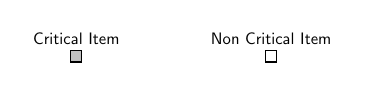
\begin{tikzpicture}[scale=0.6, every node/.style={scale=0.6}]
\node [label=Critical Item,draw,fill=gray!50] (node1) {};
\node [label={[name=l] Non Critical Item},draw,fill=white] (node2) at ([xshift=4cm]node1.east){};  
\end{tikzpicture}

				\caption{\label{fig:gant}Gant Chart}
			\end{figure}
		\end{landscape}
	
\end{document}